\documentclass{article}

\usepackage{amsmath,amsfonts,amsthm,amssymb}
\usepackage{fancyhdr}
\usepackage{lastpage}
\usepackage{graphicx}
\usepackage{supertabular}
\usepackage{multirow}
\usepackage{ifthen}
\usepackage{enumerate}
\usepackage[hidelinks]{hyperref}
\usepackage{soul}

% In case you need to adjust margins:
\topmargin=-0.5in
\evensidemargin=0in
\oddsidemargin=0in
\textwidth=6.5in
\textheight=9.0in
\headsep=0.25in

% Homework Specific Information
\newcommand{\hmwkTitle}{Project Report 2}
\newcommand{\hmwkDueDate}{March 17th, 2014}
\newcommand{\hmwkClass}{42-731}
\newcommand{\hmwkAuthor}{Alex Sun Yoo, Michael Nye, Ozan Iskilibli}
\newcommand{\hmwkEmail}{ayoo, mnye, oiskilib}
\newcommand{\hmwkCollaborators}{}
\newcommand{\bigspace}{\vspace{.25in}}

% Tools for formatting questions
\newcommand{\question}[1] {\vspace{.25in} \hrule\vspace{0.5em}
\noindent{\bf #1} \vspace{0.5em}
\hrule \vspace{.10in}}
\renewcommand{\part}[1] {\vspace{.10in} {\bf (#1)}}

% Setup the header and footer
\pagestyle{fancyplain}
\lhead{\fancyplain{}{\hmwkAuthor \\ \hmwkEmail}}
\chead{\fancyplain{}{\textbf{\hmwkTitle}}}
\rhead{\fancyplain{}{\hmwkClass \\ Due:\ \hmwkDueDate}}
\lfoot{}
\cfoot{}
\rfoot{Page\ \thepage\ of\ \pageref{LastPage}}
\renewcommand\headrulewidth{0.4pt}
\renewcommand\footrulewidth{0.4pt}

% Format paragraphs to have spacing instead of indents
\setlength{\parindent}{0pt}
\setlength{\parskip}{5pt plus 1pt}

% This is used to trace down (pin point) problems
% in latexing a document:
%\tracingall

\renewcommand{\arraystretch}{1.5}

%%%%%%%%%%%%%%%%%%%%%%%%%%%%%%%%%%%%%%%%%%%%%%%%%%%%%%%%%%%%%

\begin{document}

\thispagestyle{plain}
\begin{center}
{\Large \hmwkClass\ \hmwkTitle} \\
\hmwkAuthor \\
\hmwkEmail \\
\ifthenelse{\equal{\hmwkCollaborators}{}}{}{Collaborators: \hmwkCollaborators\\}
Due: \hmwkDueDate\\
\end{center}
%%%%%%%%%%%%%%%%%%%%%%%%%%%%%%%%%%%%%%%%%%%%%%%%%%%%%%%%%%%%%

\question{Part 1: Particle Feature Detection}

\textbf{B.2.1}

When running the script, a rectangle is manually selected by the user. It is
assumed to contain only background, and simple statistics are calculated.

\textbf{B.2.2}

Using a 5x5 mask detects noticeably fewer local extrema than using a 3x3 mask,
as shown in Figures ~\ref{fig:extrema_3} and ~\ref{fig:extrema_5}. This is
because with a larger mask, the tested point is compared with a larger area of
neighboring points, reducing its chances of being classified as a local
extrema.

The minima that are detected in one and not the other appear mostly in the
background region of the image, and not in the strip of particles we are
actually attempting to locate. This suggests the larger mask is better at
rejecting false positives.

\begin{figure}[h]
\centering
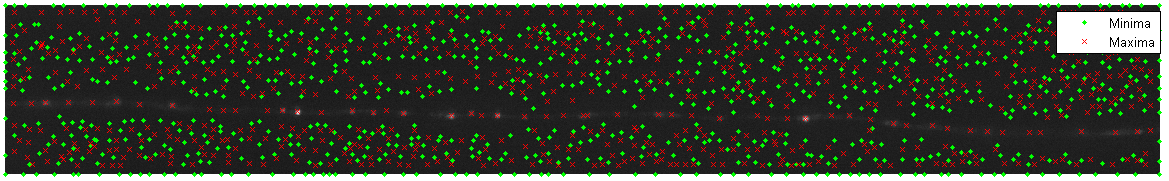
\includegraphics[width=16cm]{figures/extrema_mask_3.png}
\caption{Local Extrema (3x3 mask)}
\label{fig:extrema_3}
\end{figure}

\begin{figure}[h]
\centering
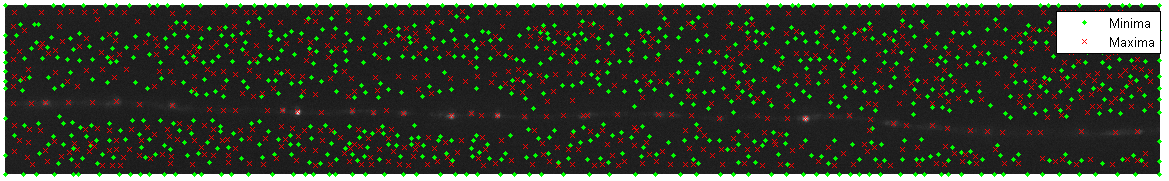
\includegraphics[width=16cm]{figures/extrema_mask_5.png}
\caption{Local Extrema (5x5 mask)}
\label{fig:extrema_5}
\end{figure}



\textbf{B.2.3}

Detected local maxima and minima in part B.2.2 is further processed by Delaunay Triangulation\cite{delaunaywiki}\cite{delaunaymathworks} as the next step. Delaunay Triangulation is method, that creates sets of triangles from given data points, whose circumcircles do not contain any vertices of neighboring triangles. In addition, this method targets to maximize the smallest angle in each created triangle. If the local minima are triangulated, then the local maxima could be assigned to each triangle evidently, eliminating some of the local maxima further. That is to say, if a Delaunay Triangle of local minima contain more than 1 local maxima, only the local maxima that has the highest intensity is accepted and rest is assumed artifacts.

When implementing this part, the \emph{DelaunayTri} class is used, as it was a built-in function in MATLAB. After that, the maxima that fall into each triangle are found. For this purpose, the matrix of local maxima and each minima triangle are swept with \emph{inpolygon}, also already available in MATLAB. This function returns the maxima that are inside or on top of the triangle vertices. Finally, among the found local maxima, the one with the highest intensity is stored as the \emph{associated local maxima} for each triangle. The triangles and their associated local maxima are shown in Figure \ref{fig:assocLocal}.

\begin{figure}[h]
\centering
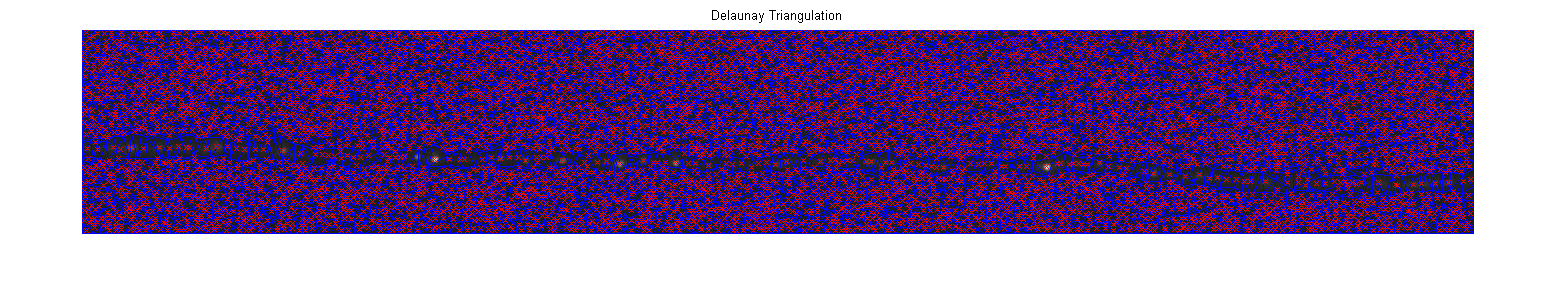
\includegraphics[width=16cm]{figures/assocLocalExtrema.png}
\caption{Associated local minima and maxima, where the minima are located at Delaunay Triangle corners and maxima are tagged with red crosses.}
\label{fig:assocLocal}
\end{figure}



\textbf{B.2.4}
 
The associated maxima found by Delaunay Triangulation method previously are further investigated in this part, in order to quantify a level of confidence for the detected particles. The question allowed to remove the speckle intensity variation term ($\sigma^2(I_L)$) in equation (4) of reference \cite{ponti}, as well as assuming that the local minima intensities' mean and variance match the cropped region's intensity mean and variance in Part B.2.1. Thanks to these simplifications, the task here reduces to comparison of background to the detected speckle in terms of intensity, with a chosen level of confidence. If this task is expressed in mathematical form, following \cite{ponti}:

\begin{align}
I_{maxima} - \mu_{BG} &= Q\cdot \sigma_{\Delta I}\\
\intertext{where $I_{maxima}$ is the intensity of the local maxima, $\mu_{BG}$ is the mean intensity of the background, $Q$ is the selection quantile for the \emph{t-test}, and the $\sigma_{\Delta I}$ is defined as}
\sigma^2_{\Delta I} &= \sigma^2(I_L) + \frac{1}{3}\sigma^2(I_{BG}) \nonumber \\
\intertext{For $\sigma^2(I_L)=0$ is given, this simplifies to}
\sigma^2_{\Delta I} &= \frac{1}{3}\sigma^2(I_{BG})
\end{align}

The only variable that is not defined by the image is the selection quantile, Q. It is, however, recommended to be chosen as a value, such that it matches the speckles that could be seen by bare eyes, when the images are shown in MATLAB. For this reason, the Q is chosen as 10. The resulting speckle detection is shown in figure \ref{fig:statMax}.

\begin{figure}[h]
\centering
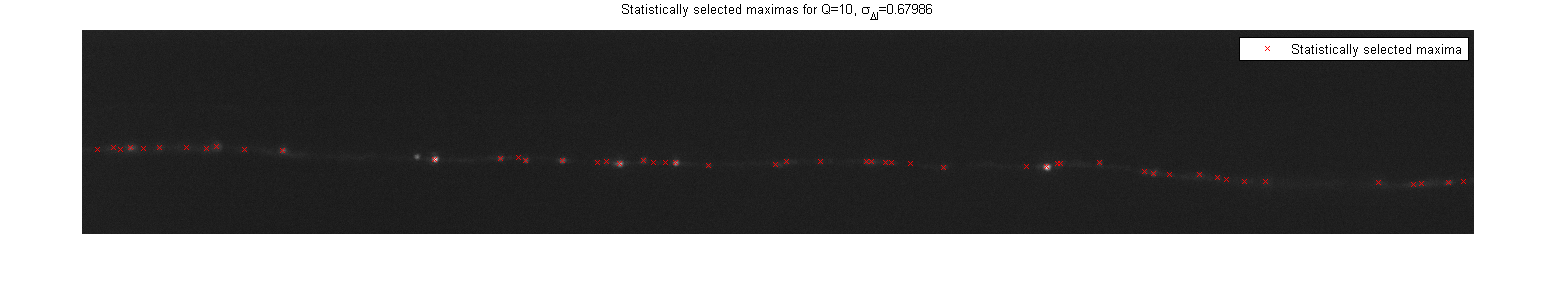
\includegraphics[width=16cm]{figures/statMax.png}
\caption{The statistically chosen maxima, tagged over the image with red crosses}
\label{fig:statMax}
\end{figure}
 
\textbf{Appendix A: Reproducing The Results}
 
The results could be reproduced as in the class presentation and this report, by setting 2 parameters in the main project m-file, ``pr2.m'', the following way.
\begin{enumerate}
\item For processing single image, set
\begin{verbatim}
Nimages = 1;
\end{verbatim}
If the figures are desired to be popping out in MATLAB, set boolean variable `plotting' from `false' to
\begin{verbatim}
plotting = true;
\end{verbatim}
\item For batch processing the image set, recommended setting is
\begin{verbatim}
Nimages = numel(images);
plotting = false;
\end{verbatim}
The MATLAB environment files in `.mat' format are stored in the `mat\_files' directory in the project root.
\end{enumerate}
 



\pagebreak
\question{Part 2: Sub-pixel Resolution Particle Detection}

\textbf{B.3.1}

Synthetic image generation is largely similar to the process used by Cheezum et al.\cite{cheezum}. First, a list of maxima are used to generate single pixel impulses. The intensity of these impulses is set to the intensity of the original image at the locations of the maxima. The image is then filtered using a Gaussian kernel to simulate the main lobe of our point spread function, and Gaussian white noise is added on top of the image.

The levels of our white noise was chosen based on the computed background statistics from part B.2.1. The results of this process can be seen in Figure \ref{fig:syntheticImage}; it closely resembles the actual image it was generated from.

\begin{figure}[h]
\centering
% TODO: replace this with a sample synthetic image
%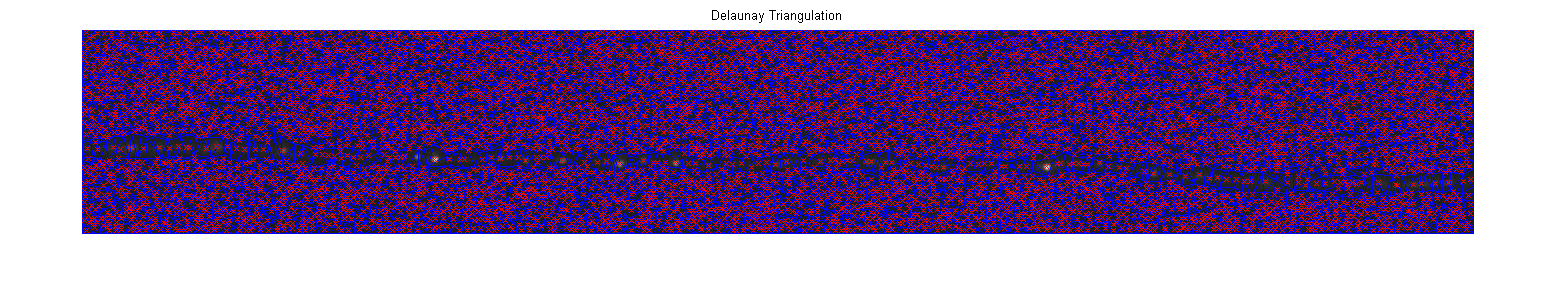
\includegraphics[width=16cm]{figures/assocLocalExtrema.png}
\caption{A sample synthetic image, and the original image it was generated from}
\label{fig:syntheticImage}
\end{figure}


\textbf{B.3.2}



\pagebreak
\begin{thebibliography}{9}
\fontsize{10pt}{12pt}\selectfont
\raggedright

    \bibitem{ponti}
        A. Ponti, P. Vallotton, W. C. Salmon, C. M. Waterman-Storer, and G.
        Danuser, \ul{Computational analysis of F-actin turnover in cortical
        actin meshworks using fluorescent speckle microscopy}, {\em Biophysical
        Journal}, 84:3336-3352, 2003.

    \bibitem{cheezum}
        M. K. Cheezum, W. F. Walker, and W. H. Guilford, 
        \ul{Quantitative comparison of algorithms for tracking single 
        fluororescent particles}, {\em Biophysical Journal}, 81:2378- 2388, 2001.

    \bibitem{delaunaywiki}
        Wikipedia -- Delaunay triangulation
        \url{http://en.wikipedia.org/wiki/Delaunay_triangulation}
    
    \bibitem{delaunaymathworks}
        Mathworks -- Delaunay triangulation
        \url{http://www.mathworks.com/help/matlab/ref/delaunay.html}

\end{thebibliography}


%%%%%%%%%%%%%%%%%%%%%%%%%%%%%%%%%%%%%%%%%%%%%%%%%%%%%%%%%%%%%

\end{document}

%%%%%%%%%%%%%%%%%%%%%%%%%%%%%%%%%%%%%%%%%%%%%%%%%%%%%%%%%%%%%
